\section{Fundamentals of Sound}
\begin{frame}{}
    \LARGE \textbf{Fundamentals of Sound}
\end{frame}

\begin{frame}{What is Sound?}
    \begin{figure}
        \centering
        \fetchconvertimage{https://letstalkscience.ca/sites/default/files/styles/x_large/public/2020-01/Sound_waves_and_particles.png}{images/audio-nlp/sound-waves.png}{width=\textwidth,height=0.6\textheight,keepaspectratio}
    \end{figure}
    \begin{itemize}
        % \setlength{\itemsep}{1.5em}
        \item Sound is a type of energy produced by vibrating objects.
        \item It travels through air (or other media) as waves.
        \item Sound waves are longitudinal waves, meaning the particle displacement is parallel to the direction of wave propagation.
    \end{itemize}
\end{frame}

\begin{frame}[allowframebreaks]{Fundamentals of Sound: Physics Concepts}
    \begin{figure}
        \centering
        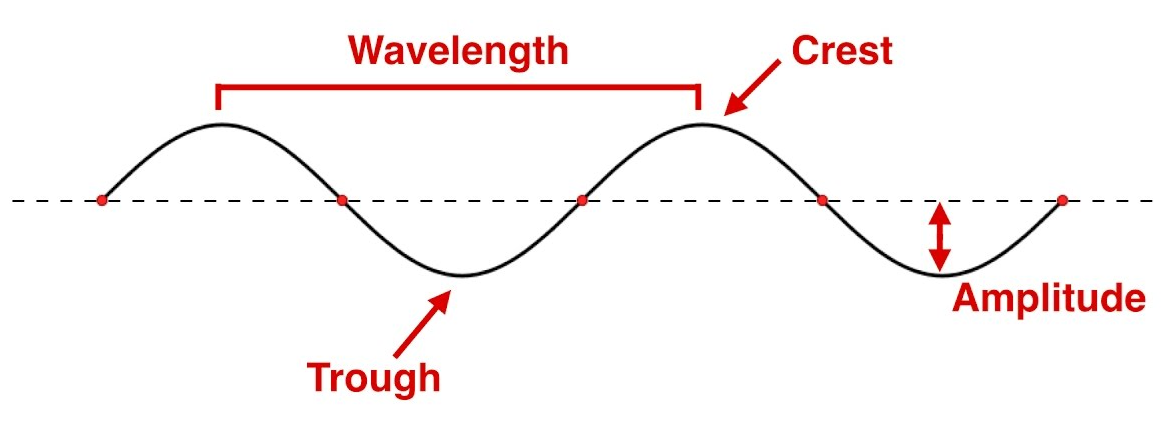
\includegraphics[width=0.6\textwidth]{images/audio-nlp/sound-props.png}
    \end{figure}
    \begin{itemize}
        \item \textbf{Waveform} $x(t)$: The shape of the sound wave, representing how air pressure changes over time.
        \item \textbf{Frequency}: Number of cycles (oscillations) per second, measured in Hertz (Hz). Determines the pitch of the sound.
        \item \textbf{Amplitude}: The height of the wave, representing the loudness or intensity of the sound.
        \item \textbf{Pitch/Formants}: The perceived frequency of a sound and its resonant frequencies, respectively.
    \end{itemize}
\framebreak
    To convert an analog signal into a digital one, two main steps are used:
    \begin{itemize}
        \item \textbf{Sampling}: The process of taking measurements of the continuous signal at regular time intervals.
        \item \textbf{Quantization}: The process of rounding off the amplitude of each sample to the nearest value on a finite scale.
    \end{itemize}
    \vspace{0.5em}
    The result is a **discrete signal**, denoted as $x[n]$, which is a sequence of numbers representing the original analog signal.
\framebreak

    \textbf{Why} do we digitize signals?
    \begin{itemize}
        \item \textbf{Computer Processing}: Computers can only understand and manipulate discrete numerical values.
        \item \textbf{Reproducibility}: Digital signals can be copied and transmitted without any loss of quality.
        \item \textbf{Processability}: Digital signals are easier to process and manipulate using various algorithms for tasks such as noise reduction, filtering, and compression.
    \end{itemize}
\end{frame}

\begin{frame}[allowframebreaks]{Digitizing speech: sampling, quantization, bitrate}
    \begin{itemize}
        \item \textbf{Sampling Rate} ($f_s$): The number of samples taken per second, measured in Hertz (Hz) or kilohertz (kHz). Common values include 16 kHz for speech and 44.1 kHz for music.
        \item \textbf{Nyquist--Shannon Sampling Theorem}: States that to perfectly reconstruct a continuous signal, the sampling rate ($f_s$) must be at least twice the maximum frequency ($f_{\max}$) of the signal.
        $$f_s \ge 2f_{\max}$$
        Failing to meet this condition can cause \textbf{aliasing}, where high frequencies are incorrectly represented as lower frequencies. The Nyquist limit, also known as the Nyquist frequency, is defined as half of the sampling rate:
        $$f_{\text{Nyq}} = \frac{f_s}{2}$$
        \item \textbf{Quantization}: The process of mapping continuous amplitude values to a finite set of discrete levels. This process introduces \textbf{quantization noise}, which is a form of error.
    \end{itemize}
    \begin{center}
        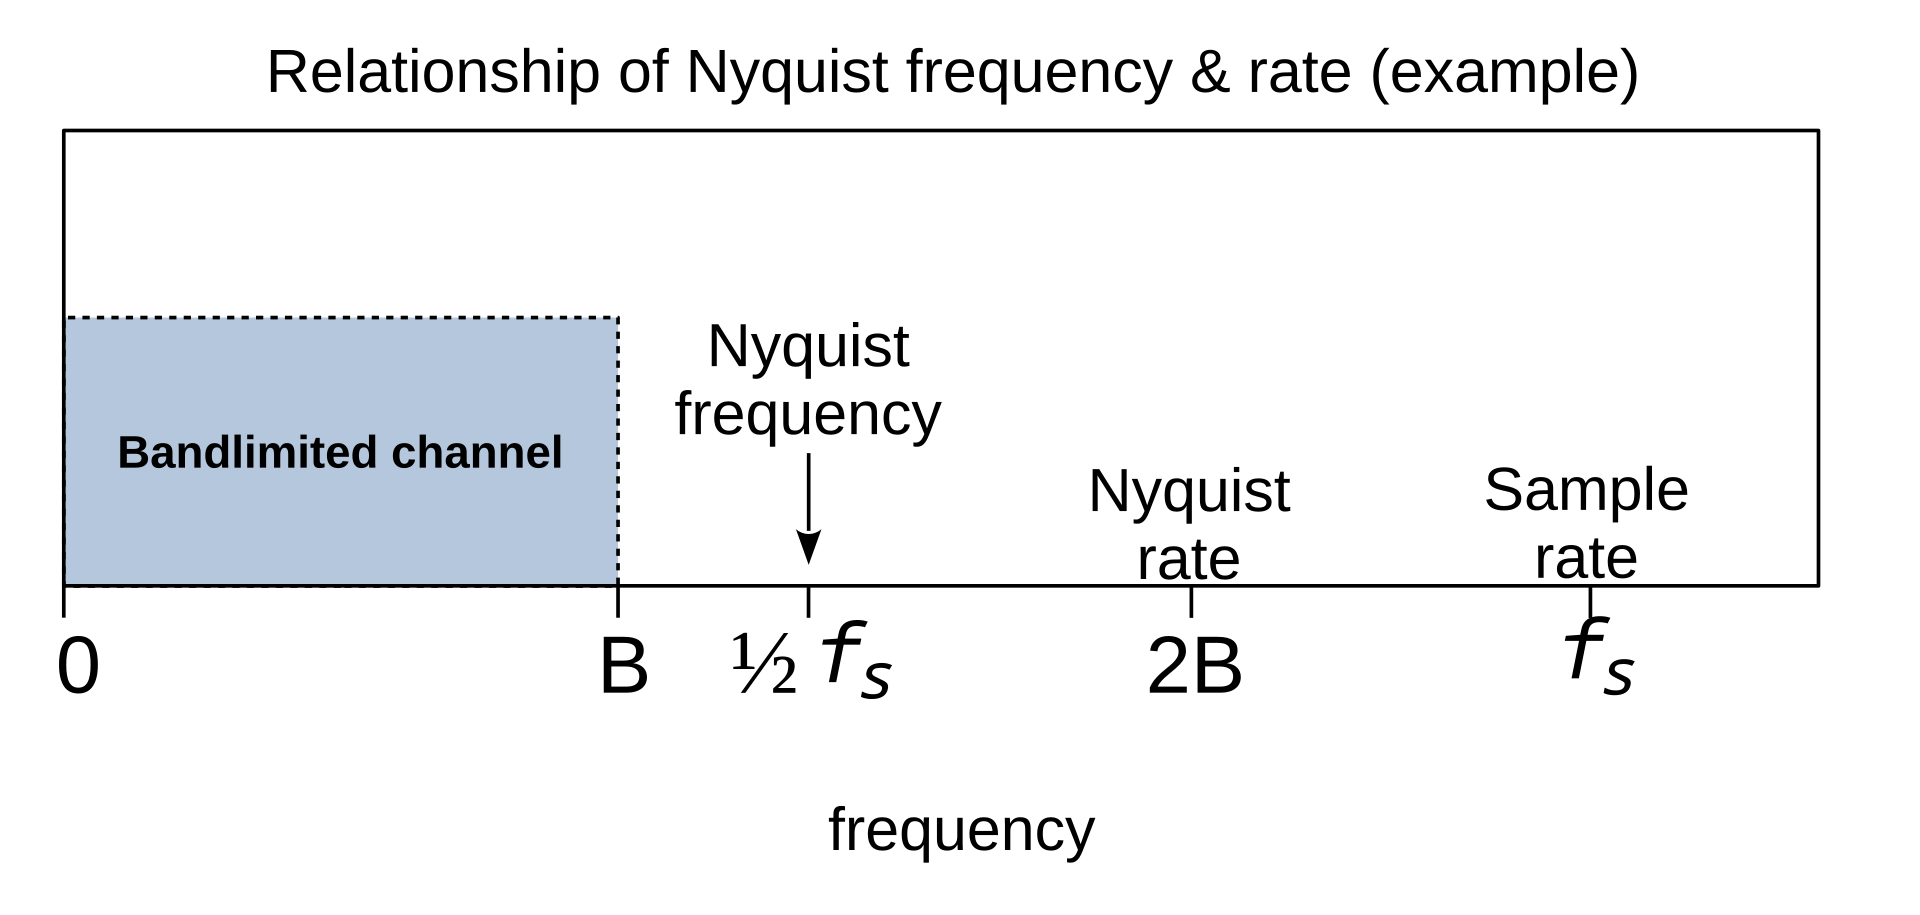
\includegraphics[width=\textwidth,height=0.5\textheight,keepaspectratio]{images/audio-nlp-eval/nyquist.png}
    \end{center}
\framebreak
    \begin{itemize}
        \item \textbf{Aliasing}: If the sampling rate is too low, higher frequencies are misrepresented as lower frequencies, causing distortion. 
        \begin{center}
            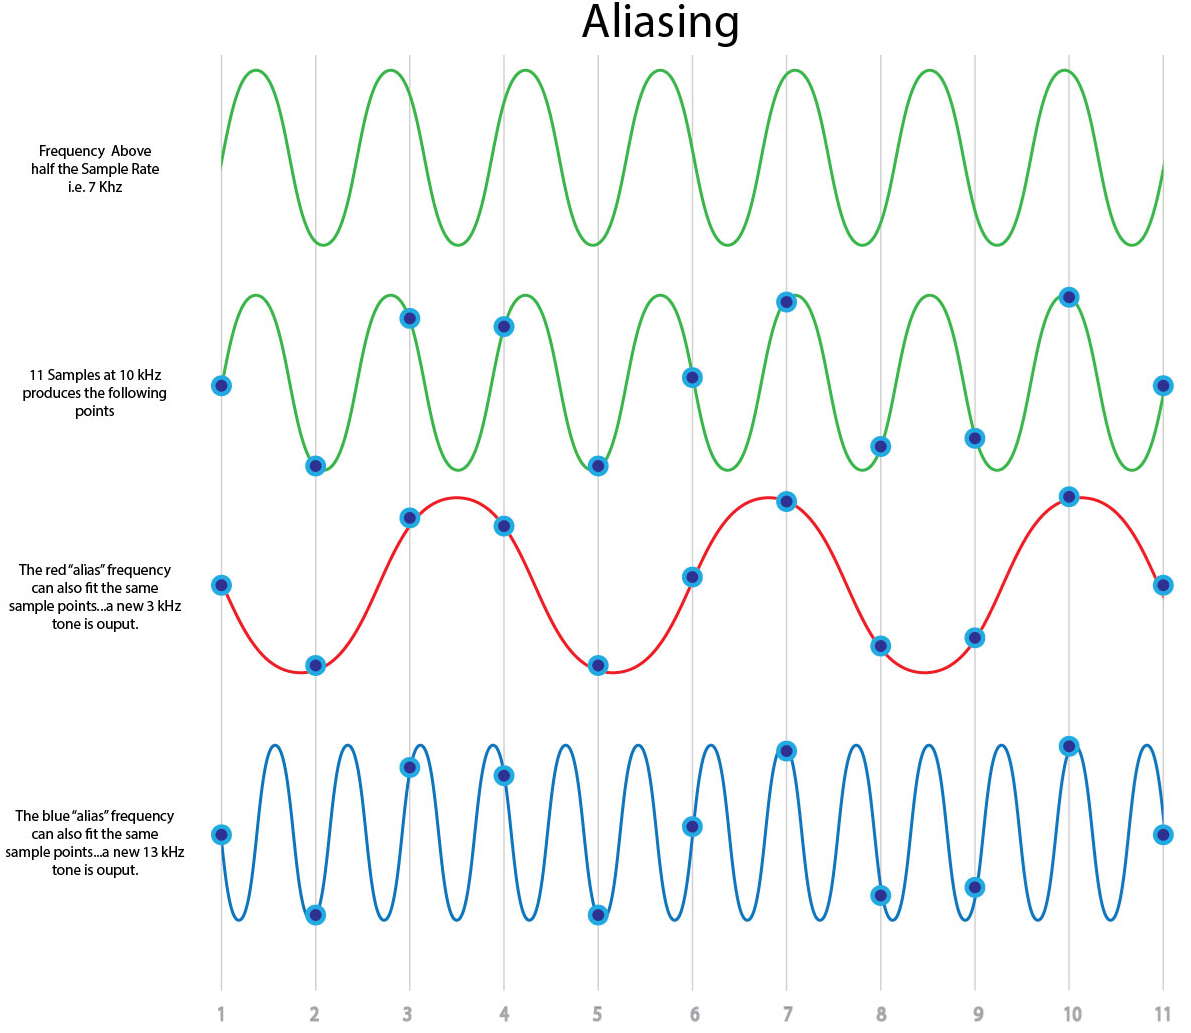
\includegraphics[width=\textwidth,height=0.9\textheight,keepaspectratio]{images/audio-nlp/aliasing.png}
        \end{center}
    \end{itemize}
\framebreak
    \begin{itemize}
        \item \textbf{Bit Depth}: Common depths include 8-bit (256 levels), 16-bit (65,536 levels), and 24-bit (16.7 million levels). Higher bit depth allows for more precise representation of amplitude.
        \item \textbf{Bitrate}: The amount of data processed per second, calculated as:
        \[
            \text{Bitrate} = \text{Sampling Rate} \times \text{Bit Depth} \times \text{Number of Channels}
        \]
        For example, a stereo audio file with a sampling rate of 44.1kHz and a bit depth of 16-bit has a bitrate of:
        \[
            44,100 \times 16 \times 2 = 1,411,200 \text{ bits per second} = 1.4112 \text{ Mbps}
        \]
    \end{itemize}
\end{frame}